\documentclass[11pt,a4paper]{article}
\usepackage[utf8]{inputenc}
\usepackage[francais]{babel}

\usepackage{amsmath}
\usepackage{amsfonts}
\usepackage{amssymb}
\usepackage{graphicx}
\usepackage[left=2cm,right=2cm,top=2cm,bottom=2cm]{geometry}

\title{Écoulements biologiques}
\author{Tiago Lobato Gimenes \\ Chongmo Liu}

\begin{document}

\maketitle

\section*{Introduction}

TODO: ecrire introduction

\section{Problème proposé}

Le problème proposé a été d'étudier les écoulements biologiques, plus précisément, l'écoulement sanguin dans des petites artères.
 
Le modèle mathématique proposé pour résoudre ce problème a eu une évolution au cours du modal. Premièrement nous avons commencé avec un modèle simple d'écoulement d'un fluide incompressible dans un tube avec des parois fixes. Nous avons aussi supposé que le nombre de Reynolds de  l'écoulement est petit et que les forces volumiques sont négligeables, ce que nous a permit d'utiliser le modèle suivante:
\begin{equation}
\begin{aligned}
& -\nu \Delta u + \nabla p = 0 \\
& -\mathrm{div}\;u = 0 \label{Stokes}
\end{aligned}
\end{equation}

Nous avons décidé, d'abord, de commencer par simulant le problème \ref{Stokes} dans le rectangle $\Omega = \{(x,y) \in \mathbb{R}^2 \;t.q\; 0 \leq x \leq L, \; -R/2 \leq y \leq R/2\}$. Les conditions au limites du problème que nous avons utilisé ont été:
\begin{equation}
\begin{aligned}
& \underline{u}(x,-R/2) = \underline{0} \\
& \underline{u}(x, R/2) = \underline{0} \\
& \underline{u}(0,y) = \left(-\frac{1}{2}\left(y-\frac{R}{2}\right)^2 + \frac{R}{4}^2, 0\right) \\
& \nu\frac{\partial\underline{u}}{\partial n}(L,y) = p\underline{n}
\end{aligned} \label{LimitesClassiques}
\end{equation}

La formulation variationnelle du problème \ref{Stokes} avec les conditions \ref{LimitesClassiques} devient, donc, la suivante:
\begin{equation}
\nu \int\limits_\Omega \nabla \underline{u} \nabla \underline{v} \;\mathrm{d}\Omega - \int\limits_\Omega p\nabla v \; \mathrm{d}\Omega = 0
\end{equation}

où $v$ est une fonction nulle sur touts les bords du rectangle $\Omega$ sauf sur la bord où $x = L$.

En faisant la simulation du problème \ref{Stokes} avec les conditions aux limites \ref{LimitesClassiques} nous avons comme résultat:
\begin{figure}[h]
\centering
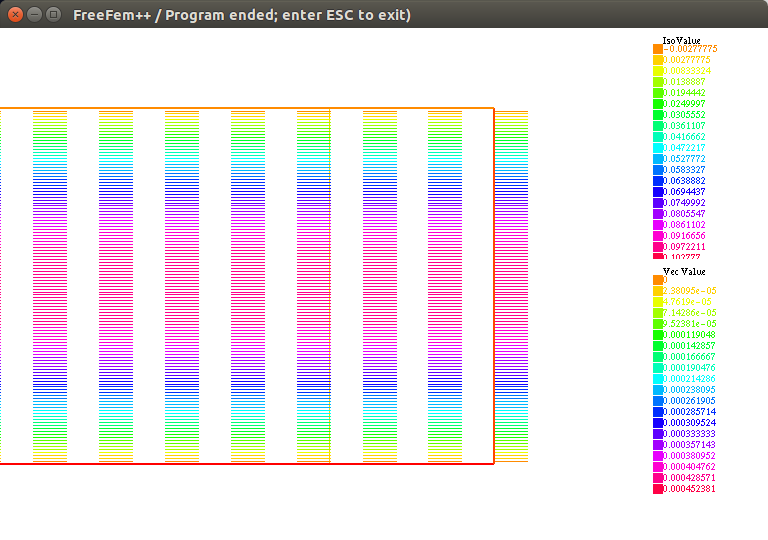
\includegraphics[scale=0.4]{StokesConditionsClassiques.png}
\caption{Vision de la vitesse pour le problème \ref{Stokes} avec les conditions \ref{LimitesClassiques}}
\end{figure}

\begin{figure}[h]
\centering
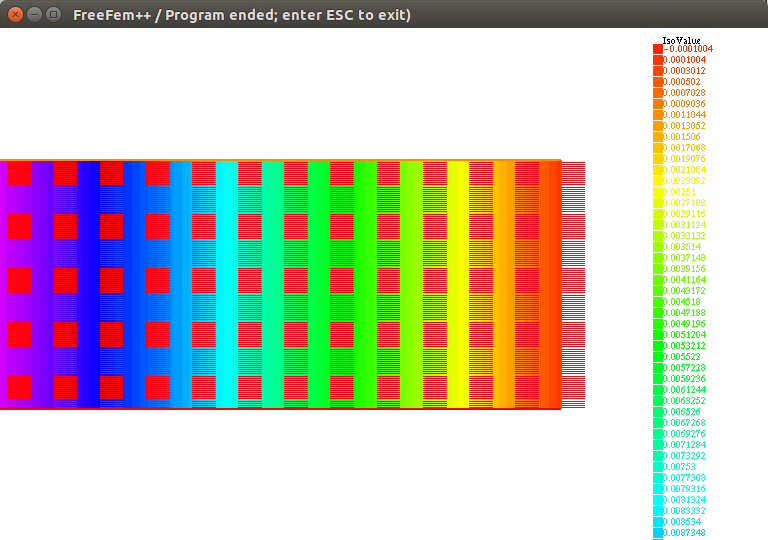
\includegraphics[scale=0.4]{StokesConditionsClassiquesPression.png}
\caption{Vision du gradient de pression pour le problème \ref{Stokes} avec les conditions \ref{LimitesClassiques}}
\end{figure}
\end{document}